\section{Grundlagen}
Dieses Kapitel führt die theoretischen und methodischen Grundlagen ein, die für das Verständnis der im Folgenden vorgestellten 
Reglerarchitekturen und Bildverarbeitungsverfahren notwendig sind. Zunächst wird die PID-Regelung als klassischer Vertreter der 
Regelungstechnik erläutert und ihre Eignung zur Stabilisierung des Balance-Problems des Fahrrads diskutiert. 
Anschließend folgt eine Einführung in das Prinzip der modellprädiktiven Regelung (MPC), die eine vorausschauende Berechnung von 
Stellgrößen erlaubt. Abschließend werden die Grundlagen der Objekt­erkennung 
mit YOLO sowie der Bildsegmentierung vorgestellt, um die visuelle Wahrnehmung und Spurführung des autonomen Fahrrads zu ermöglichen.

\subsection{PID-Regelung – Prinzip und Eignung für das Balance-Problem}

Die Proportional‑Integral‑Differential (PID)‑Regelung ist der am weitesten verbreitete Ansatz der klassischen Regelungstechnik. 
Ein PID‑Regler ermittelt die Stellgröße \(u(t)\) aus dem Fehler \(e(t)\) zwischen Sollwert \(\text{SP}\) und dem gemessenen Istwert \(\text{PV}\) nach
\begin{equation}
  u(t)=K_{\mathrm{P}}\,e(t) + K_{\mathrm{I}}\int_0^t e(\tau)\,\mathrm{d}\tau + K_{\mathrm{D}}\frac{\mathrm{d}e(t)}{\mathrm{d}t}
  \label{eq:pid}
\end{equation}
wobei \(K_{\mathrm{P}}\), \(K_{\mathrm{I}}\) und \(K_{\mathrm{D}}\) die Verstärkungsparameter für proportionale, integrale und 
derivative Anteile sind.  Der proportionale Anteil erzeugt eine Stellgröße, proportional zur momentanen 
Fehlergröße und reduziert so die Anstiegszeit.  Der Integrator akkumuliert den Fehler und eliminiert stationäre Abweichungen, kann 
aber langsame Dynamik verursachen \cite{apmonitor_pid}.  Die Derivative wirkt der Änderung des Fehlers entgegen und dämpft dadurch Überschwinger. Sie 
erhöht jedoch die Empfindlichkeit gegenüber Messrauschen, weshalb in vielen Anwendungen filternde Maßnahmen erforderlich sind.

PID‑Regler werden eingesetzt, wenn eine robuste und einfach implementierbare Rückführung 
gefordert ist und das Systemverhalten 
hinreichend durch lineare Modelle beschrieben werden kann.  In der Literatur wird die PID‑Regelung häufig als Standardlösung für 
nicht integrierende Prozesse bezeichnet.  Ihre Parametrierung erfordert eine sorgfältige Abwägung zwischen 
Ansprechverhalten und Stabilitätsreserve. Eine Erhöhung des proportionalen Anteils verringert die Regelabweichung, kann aber zu
 Instabilitäten führen. Ein zu hoher Integrationsanteil kann Integrator‑Windup verursachen, die wiederum zu Instabilitäten führen kann.

Beim selbstbalancierenden Fahrrad lässt sich die Balanceproblematik auf das klassische 
inverses-Pendel‑Problem zurückführen.  
Ein Rad, dessen Schwerpunkt über der Aufstandsfläche liegt, befindet sich in einem instabilen Gleichgewicht, wodurch kleinste Störungen 
zum Kippen führen.  Um das System aufrecht zu halten, muss der Regler in Echtzeit Stellmomente ansetzen, die den kippspezifischen 
Drehmomenten entgegenwirken.  Die Anforderungen an geringe Latenz und hohe Abtastrate werden etwa beim inversen Pendel mit Updatefrequenzen 
von mehreren Kilohertz umgesetzt.  Dies verdeutlicht, dass auch beim Fahrrad eine schnelle Regelungsschleife erforderlich ist, wie sie 
beispielsweise in den Bachelorarbeiten von Karabila und Zander implementiert wurde. Beide Arbeiten basieren auf P‑ bzw. PID‑Reglern, die den 
Neigungswinkel mittels IMU messen und über den Lenkmotor oder den Antrieb korrigieren \cite{concurrent_rt_inverted_pendulum}.

Insgesamt ist die PID‑Regelung für das Balance‑Problem des autonomen Fahrrads wegen ihrer geringen Komplexität und Rechenlast, der 
einfachen Implementierung auf Mikrocontrollern sehr gut geeignet.  Die Nichtlinearität 
des Fahrverhaltens und die starken Störmomente durch Schräglagen erfordern jedoch eine sorgfältige Abstimmung der Parameter und 
gegebenenfalls Erweiterungen wie Anti‑Windup‑Mechanismen oder Filterung der derivativen Komponente, um die Regelung stabil und performant zu halten.


\subsection{MPC-Regelung – Prinzip und Eignung für das Fahrtrichtungsproblem}
Model predictive control (MPC) nutzt ein internes Modell des Systems, um dessen zukünftiges Verhalten über einen endlichen Zeithorizont vorherzusagen.  
Auf Grundlage dieser Vorhersage und des aktuellen gemessenen bzw. geschätzten Zustands werden optimale Stellgrößen berechnet, die einen definierten 
Kostenfunktional minimieren und gleichzeitig die Systembeschränkungen einhalten.  Nach jedem Abtastintervall wird nur die erste Stellgröße angewendet
und die Optimierung mit vorwärts verschobenem Horizont neu gelöst, weshalb man auch von \emph{receding horizon control} spricht.  Zu den wesentlichen 
Vorteilen von MPC zählen die proaktive Reaktion auf künftige Störungen, die Möglichkeit nichtlineare Modelle ohne Linearisierung zu berücksichtigen 
und die explizite Berücksichtigung von physikalischen und sicherheitsrelevanten Beschränkungen.  Im Gegensatz zu reaktiven PID‑Reglern kann MPC damit 
frühzeitig gegensteuern und gleichzeitig harte Grenzen, etwa Stellweg‑ oder Geschwindigkeitsbeschränkungen, einhalten.

\begin{figure}[H]
  \centering
  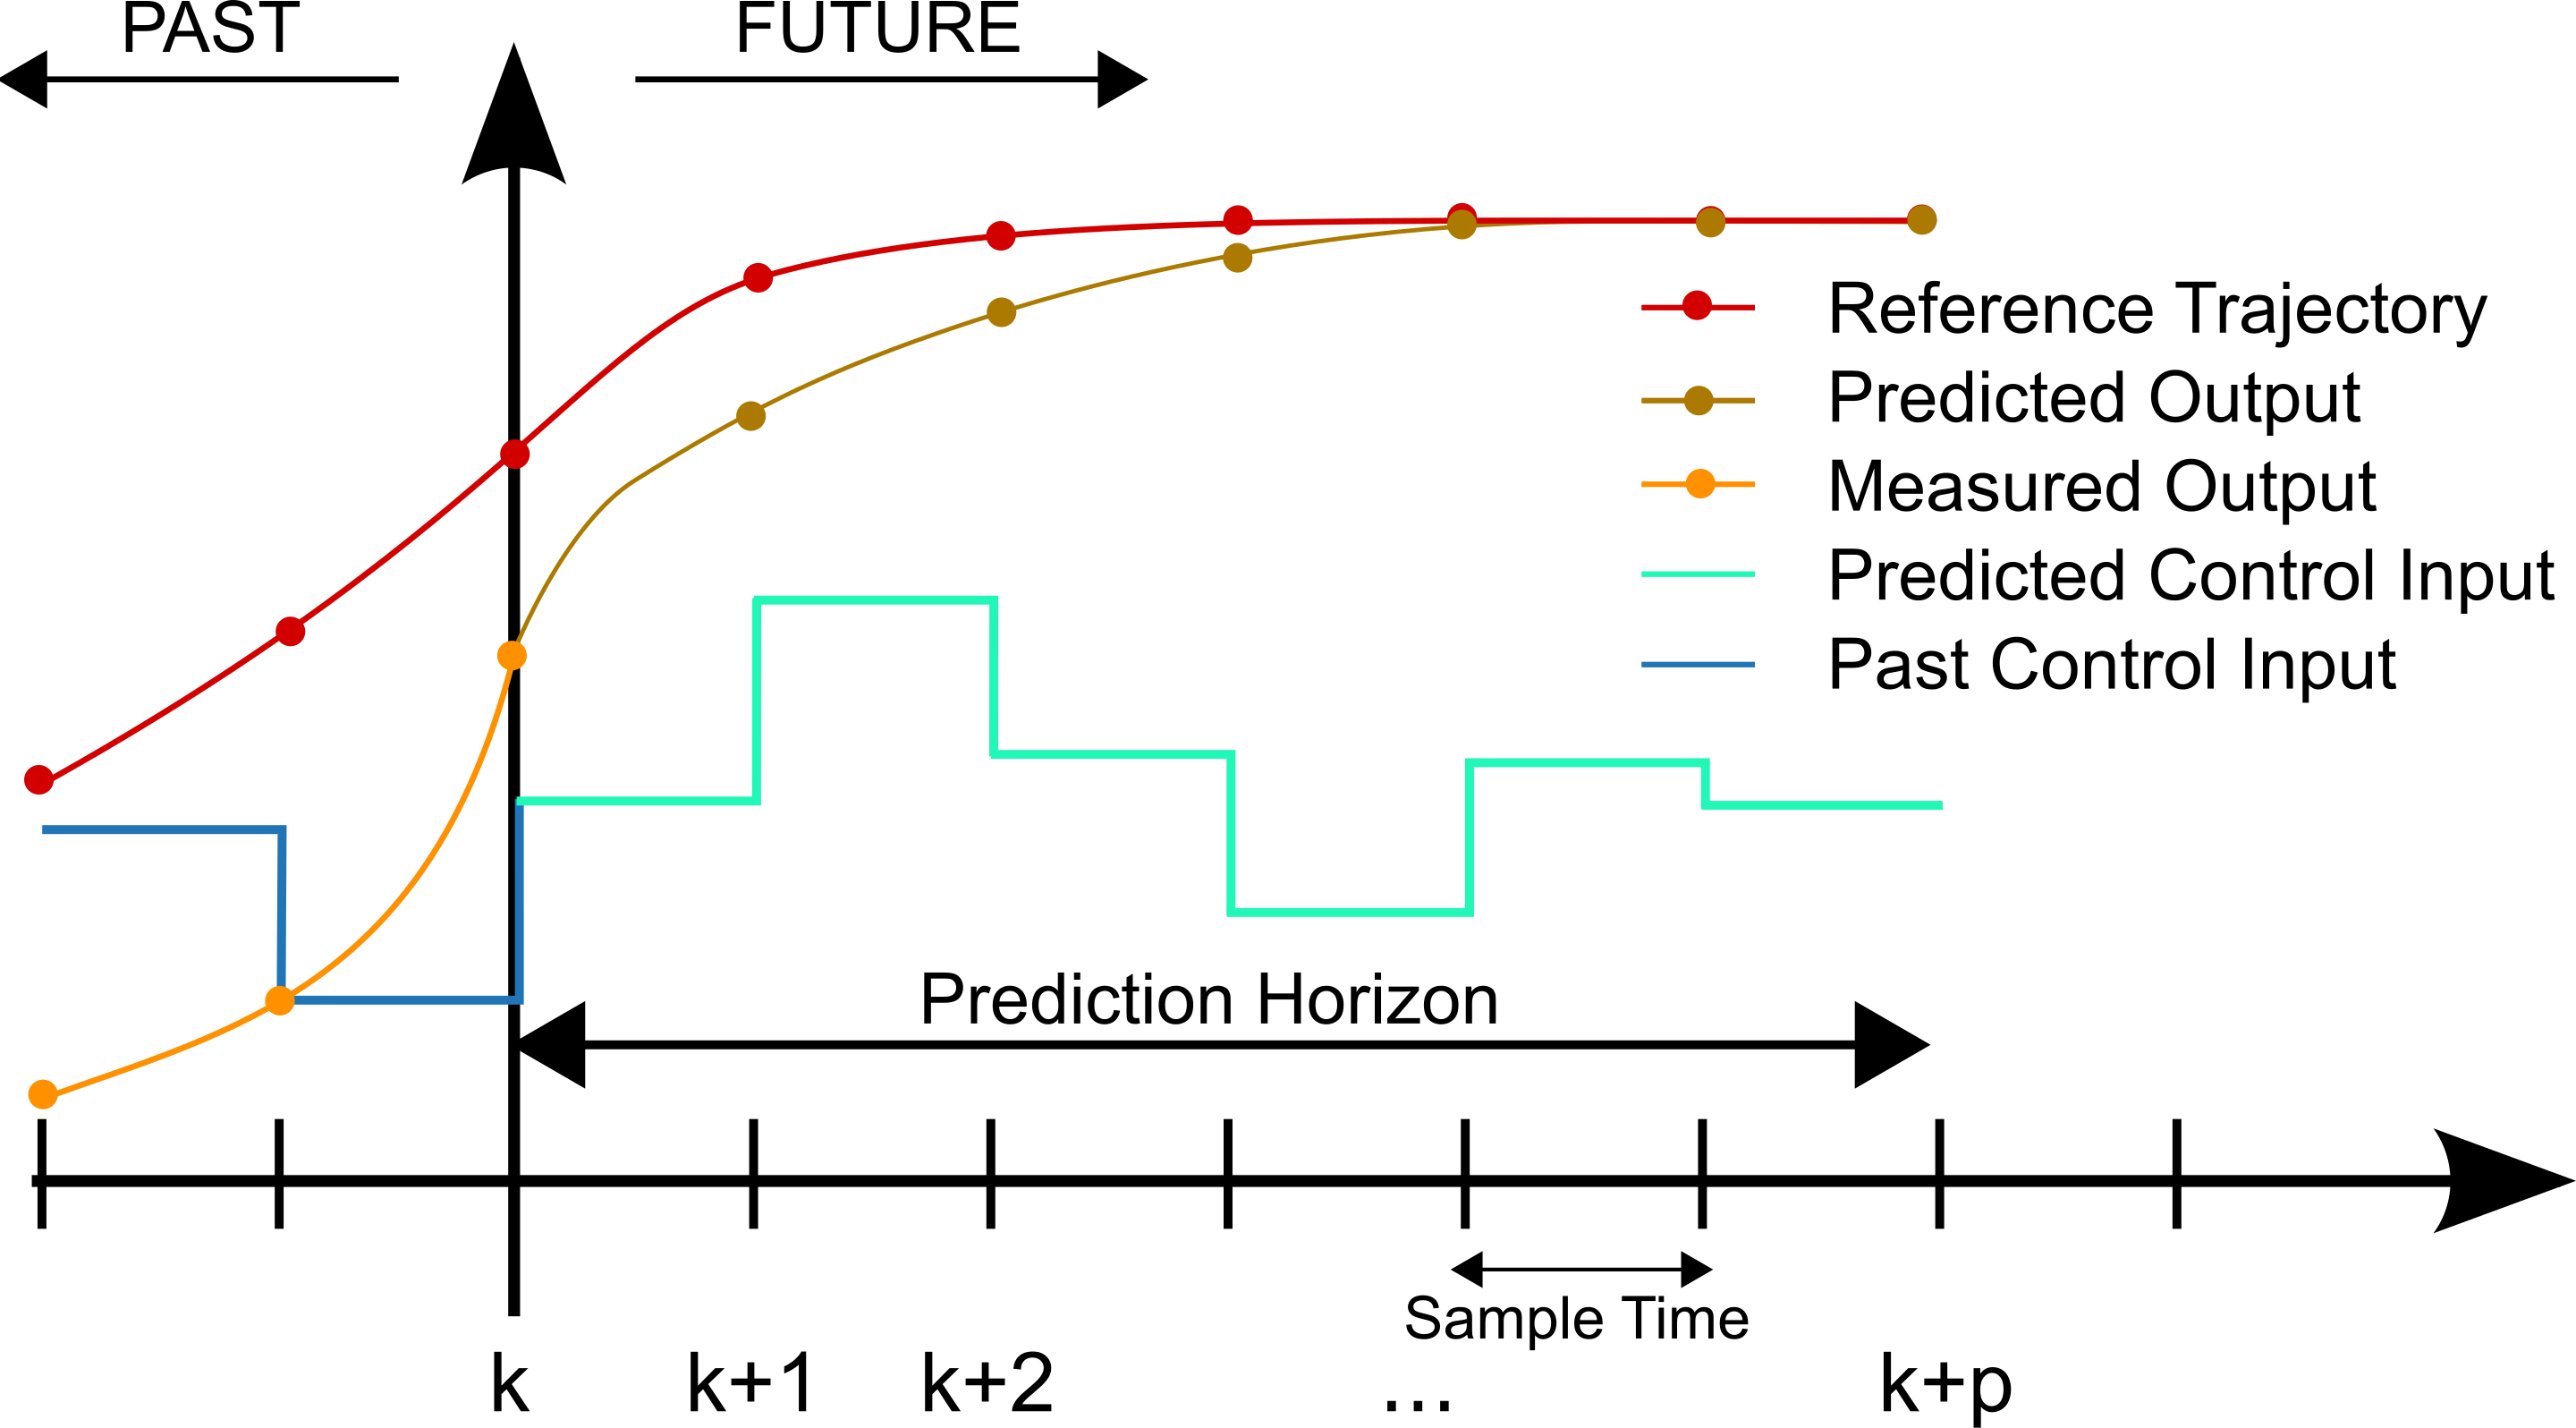
\includegraphics[width=0.8\textwidth]{figures/MPC_scheme_basic.svg.png}
  \caption{Verständnisschema der MPC-Regelung}
  \label{fig:mpc_scheme_basic}
\end{figure}

Beim selbstbalancierenden Fahrrad besteht das Fahrtrichtungsproblem darin, aus Kamerainformationen einen Sollkurs abzuleiten und das Fahrzeug 
mit begrenztem Lenkradius und Lenkrate entlang dieser Trajektorie zu führen.  Der in der Vision‑Regelung verwendete \texttt{VisionMPCController} 
modelliert das Fahrzeug als einfaches Fahrraddynamikmodell mit Zustandsvektor \(x=[x, y, v,\psi]\) für Position, Geschwindigkeit und Gierwinkel 
sowie Eingangsvektor \(u=[a,\delta]\) für Beschleunigung und Lenkwinkel.  Aus dem aktuellen Zustand und dem lateral 
gemessenen Fehler wird ein Referenzpfad erzeugt (Ziel‑Yaw proportional zum Fehler), der über einen Horizont \(T\) vorwärts projiziert wird.  
Anschließend löst der MPC ein konvexes Optimierungsproblem, das die Abweichung von diesem Pfad, die Eingangsgrößen sowie deren zeitliche 
Änderung in einer quadratischen Kostenfunktion gewichtet und durch Beschränkungen auf maximalen Lenkwinkel, Lenkrate, Geschwindigkeitsbereich 
und Beschleunigung ergänzt.  Stehen geeignete Optimierungslöser (z.\,B. \texttt{cvxpy}) zur Verfügung, werden aus diesem Problem kontinuierliche 
Stellgrößen \(\delta\in[-\delta_{\max},\delta_{\max}]\) berechnet, andernfalls fällt der Controller auf eine einfache P‑Regelung zurück.  
Vor der Weitergabe an den schnellen Balance‑Controller werden die resultierenden Lenkwinkel und Beschleunigungen normiert, geglättet und auf Änderungsraten 
begrenzt, um ruckfreie Übergänge zu gewährleisten \cite{vision_mpc_readme}. Eine spezifische erklärung der implementierten Regelung findet sich in Kapitel 5.2.

Die Eignung der MPC Regelung für das Fahrtrichtungsproblem ergibt sich aus der Vorhersagefähigkeit und der Einbeziehung von Beschränkungen.  
Das Fahrradsystem ist nichtlinear und um einer gekrümmten Spur zu folgen, muss der Regler zukünftige Kurvenverläufe 
berücksichtigen und gleichzeitig mechanische Limits (Lenkeinschlag, Lenkrate) respektieren.  MPC kann diese Randbedingungen explizit 
in das Optimierungsproblem integrieren und die Stellgrößen so wählen, dass sowohl die Trajektorienabweichung als auch der Stellaufwand 
minimiert werden.  In Yasin Girays Masterarbeit wurde der visionbasierte MPC‑Regler mit einem Horizont von \(T=3\) und den genannten 
Zuständen und Eingängen implementiert und mit Gewichten auf Zustände, Eingänge und deren Differenzen parametriert.  
Simulationen zeigten, dass das Fahrrad mithilfe des MPC gleichmäßig entlang der aus der Bildsegmentierung abgeleiteten Spur navigierte und 
dabei die mechanischen Limits einhielt.  Somit stellt MPC einen geeigneten Ansatz dar, um das autonome Fahrrad stabil und vorausschauend 
entlang einer vorgegebenen Fahrtrichtung zu steuern.

\subsection{YOLO-Grundlagen und Segmentierung} \label{chap:yolo}

You Only Look Once (YOLO) ist eine Reihe von Echtzeit‑Objekterkennungsverfahren, die auf Convolutional Neural Networks basieren.  Das ursprüngliche YOLO wurde 
2015 von Redmon et al. vorgestellt und erfordert im Gegensatz zu region‑proposal‑basierten Ansätzen nur einen Vorwärtsdurchlauf durch das Netz, um Klassen und 
Bounding Boxes für alle Objekte in einem Bild bestimmen \cite{yolo_wikipedia}.  Neuere Modelle wie YOLOv8 erweitern die ursprüngliche YOLO-Architektur. 
Sie können nicht nur Objekte erkennen, sondern auch Bilder klassifizieren und Instanzen segmentieren. Ein moderner, leichter Backbone
\footnote{Der Backbone ist das Merkmalsextraktionsnetz der Architektur. Er transformiert das Eingabebild in hierarchische, mehrskalige 
Feature-Maps, die die Grundlage für Klassifikation, Lokalisierung und Segmentierung bilden.}, ein ankerfreier 
Detektionskopf \footnote{Ankerfrei bedeutet ohne vordefinierte Ankerboxen. Der Kopf schätzt pro Bildposition direkt Objektzentren und 
Boxparameter sowie Klassenwahrscheinlichkeiten, was Hyperparameter reduziert und das Matching im Training vereinfacht.} und verbesserte 
Verlustfunktionen erhöhen Effizienz und Genauigkeit. Dadurch laufen die Modelle auf vielen Hardwareplattformen zuverlässig und schnell \cite{openmmlab_yolov8}.

Bei der Bildsegmentierung wird jedem Pixel eines Bildes ein Label zugeordnet.  Semantic Segmentation ordnet jedem Pixel eine Objektklasse zu, ohne zwischen 
einzelnen Instanzen zu unterscheiden, während Instance Segmentation jedes Pixel einer individuellen Objektinstanz zuordnet \cite{image_segmentation_wikipedia}.  
Panoptic Segmentation kombiniert beide Ansätze, indem sie sowohl die Klasse als auch die Instanz für jedes Pixel identifiziert \cite{image_segmentation_wikipedia}. 
 In der Instanzsegmentierung liefert das Netzwerk neben Bounding Boxes auch Masken, die die Form jedes erkannten Objekts abbilden.

 YOLOv8 erweitert die Objekterkennung um Instanzsegmentierung, wobei ein auf YOLACT \footnote{YOLACT steht für You Only Look At Coefficients 
 und ist ein einstufiges Verfahren zur Instanzsegmentierung. Es erzeugt Prototypmasken und kombiniert sie mit Koeffizienten zu Objektmasken} 
 basierender Kopf für jedes erkannte Objekt eine zusätzliche Maske berechnet \cite{openmmlab_yolov8}.  
 Durch diese Erweiterung kann ein Modell in einem einzigen Forward‑Pass sowohl Objekte lokalisieren als auch 
deren pixelgenauen Umrisse bestimmen.  Wie bei früheren YOLO‑Versionen werden Varianten unterschiedlicher Größe bereitgestellt (Nano, Small, Medium, Large usw.), 
um den Kompromiss zwischen Geschwindigkeit und Genauigkeit zu steuern \cite{openmmlab_yolov8}.

In dieser Arbeit wird eine YOLOv8‑basierte Segmentierung für die Umfeldwahrnehmung genutzt.  Das Modell ist auf vier Klassen trainiert: Wiese 
(„meadow“), Hindernis („obstacle“), Hauptfahrbahn („street\_main“) und Seitenfahrbahn („street\_side“), wie in Abbildung \ref{fig:yolo} zu sehen ist \cite{vision_mpc_readme}. Dabei liefert es
pro Klasse ein Pixelmasken Overlay sowie die zugehörigen Bounding Boxes.  Anschließend wird aus dem Segment „street\_main“ der laterale Fehler 
bestimmt, der als Eingang für die Pfadverfolgung dient.  Die genauen Details zur Modellauswahl, Datensatzgenerierung und Implementierung werden 
in einem späteren Kapitel beschrieben.  Hier soll lediglich hervorgehoben werden, dass die Kombination aus schneller YOLO‑Detektion und Instanzsegmentierung 
eine effiziente und genaue Grundlage für die kamerabasierte Fahrspurerkennung bildet.





\begin{figure}[H]
  \centering
  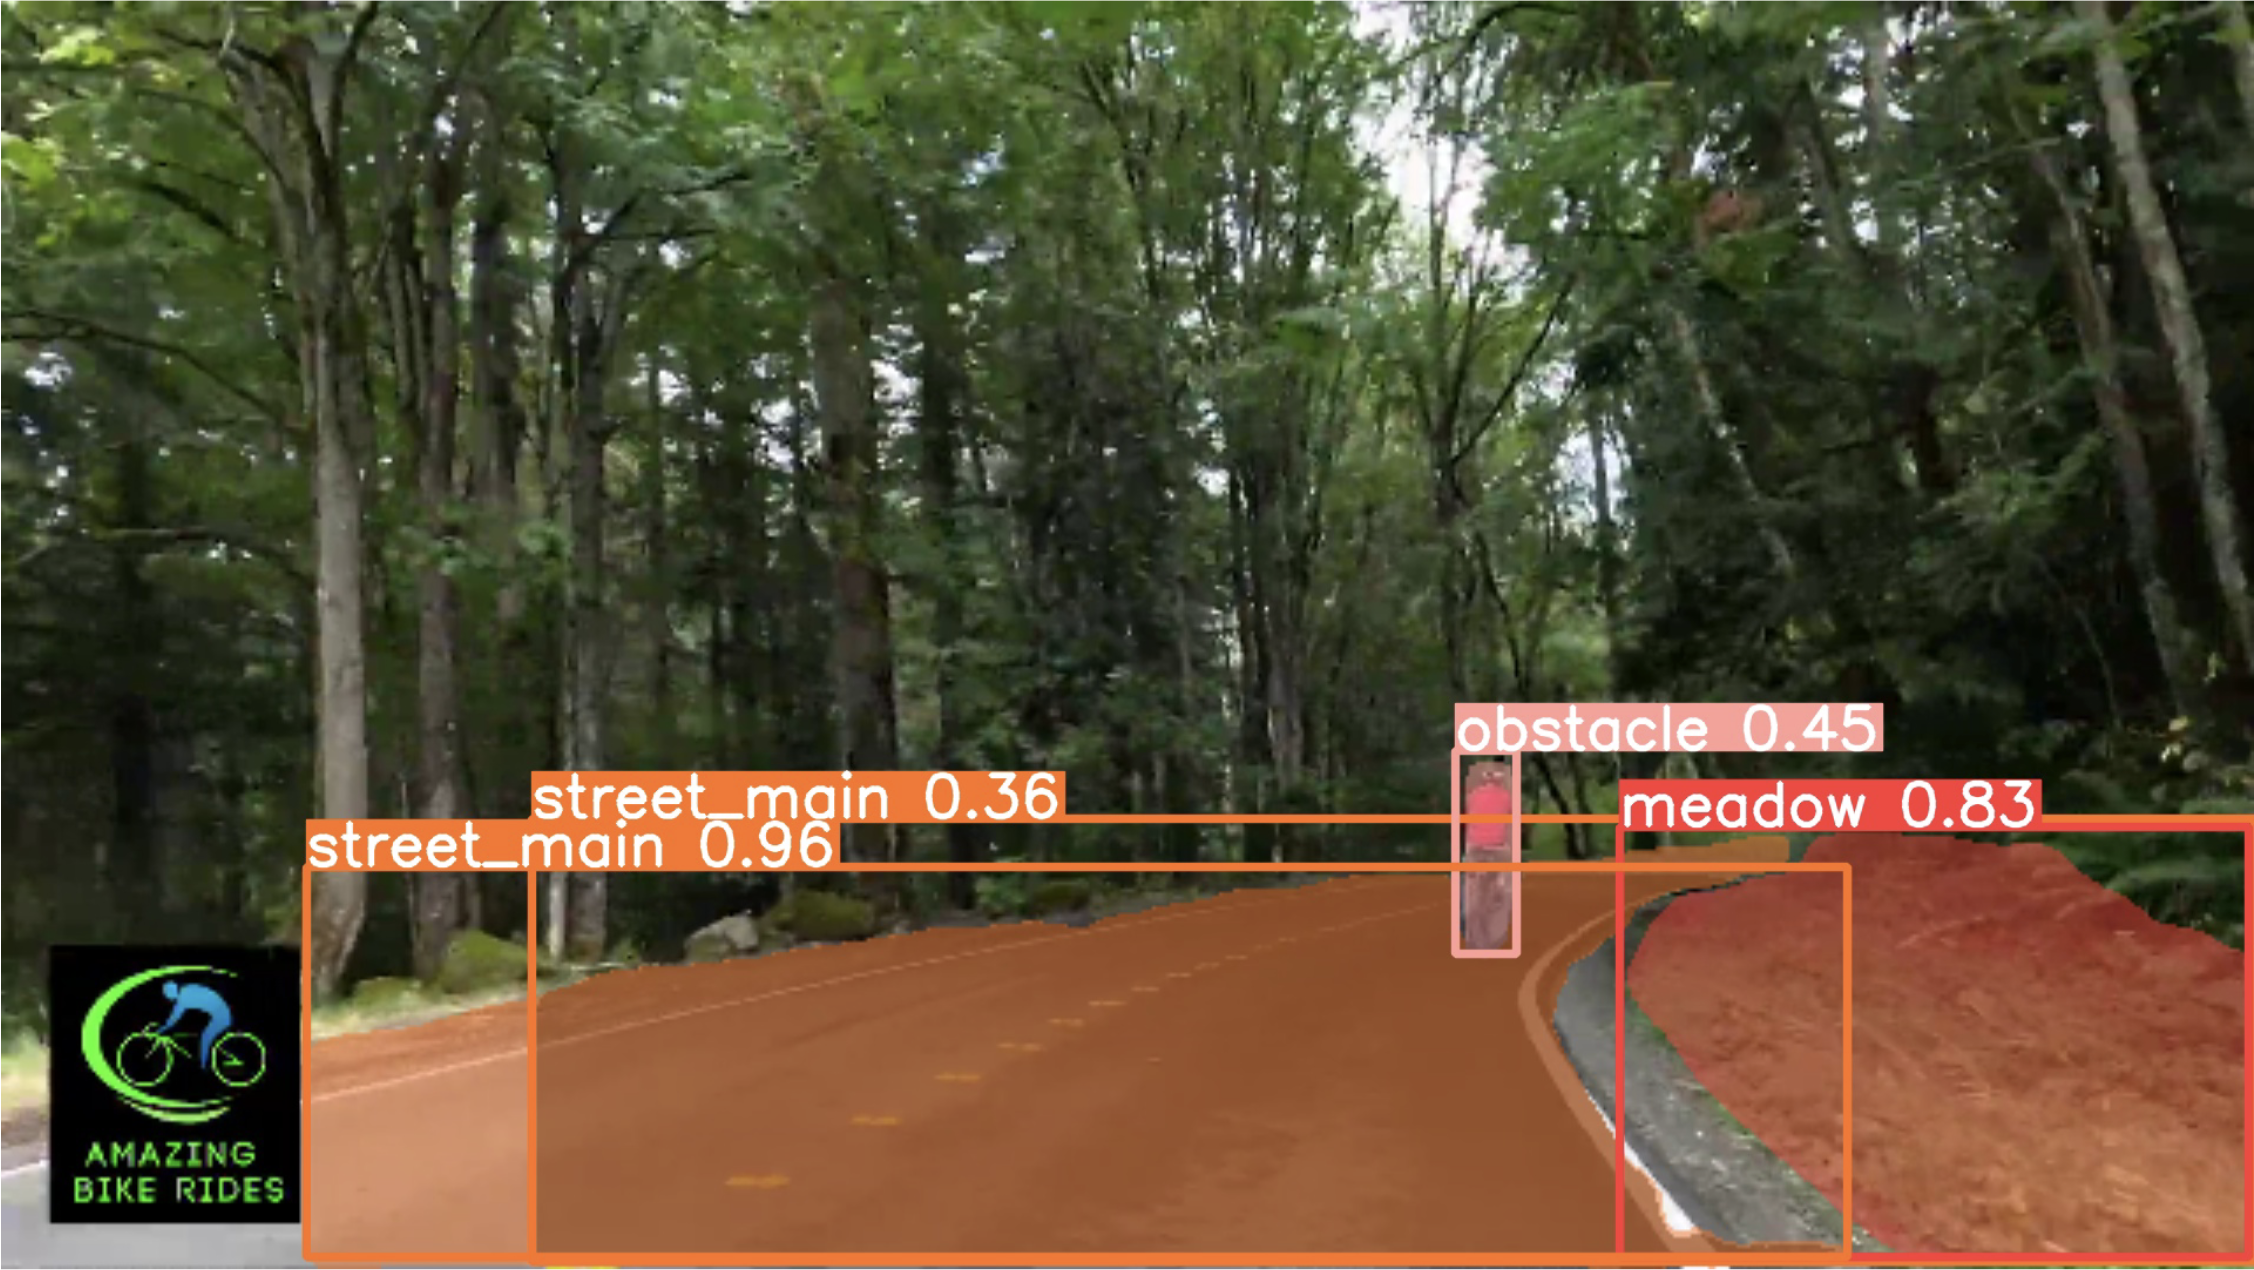
\includegraphics[width=0.8\textwidth]{figures/Yolo.png}
  \caption{YOLO-Segmentierung mit YOLOv8}
  \label{fig:yolo}
\end{figure}